\documentclass[10pt,oneside,a4paper]{article}
\usepackage[left=2cm,right=2cm,top=2cm,bottom=1cm,includeheadfoot]{geometry}
\usepackage{ngerman}
\usepackage[utf8]{inputenc}
% \usepackage{amsfonts,amssymb,amsmath,cancel,graphicx,textcomp}
\usepackage{amsfonts,amssymb,amsmath,graphicx,textcomp}
\usepackage{float}
\usepackage{color,xcolor}
\usepackage{url}
\usepackage{hyperref}
\usepackage{listings}
\usepackage{tikz}
\usepackage{fancyhdr}
\usepackage{gensymb}
\usepackage[section]{placeins}
\usetikzlibrary{arrows,shapes,snakes,automata,backgrounds,petri,positioning}

\hypersetup{
    colorlinks,
    citecolor=black,
    filecolor=black,
    linkcolor=black,
    urlcolor=black
}

\pagestyle{fancy}
\fancyhf{}
\fancyhead[L]{crash override : \\Steve Dierker, Semjon Kerner, Artur Jeske}
\fancyhead[C]{"Ubungsblatt 11}
\fancyhead[R]{Seite \thepage}
\renewcommand{\headrulewidth}{0.5pt}

% lstlisting mit Zeilennummerierung und grauen Kommentaren, Zeilenumbruch, etc. pp.
\lstset{
  numbers=left, numberstyle=\tiny, numbersep=5pt,
  tabsize=2,
  breaklines=true, breakindent=0pt, postbreak=\mbox{$\rightarrow\ \ $},
  showstringspaces=false,
  extendedchars=false,
  basicstyle=\small\ttfamily,
  commentstyle=\color{black!40},
  stringstyle=\color{black!40!blue},
  keywordstyle=\color{black!40!green}
}

% Komma Abstände bei Tausendern/Dezimalzahlen ans dt. anpassen
\mathcode`,="013B
\setlength{\parindent}{0em}
\setlength{\parskip}{0.5em}

\begin{document}
  \section{Calculate Distance to Nearest Obstacle on Lane (10 Points)}
    \begin{figure}[h]
      \centering
      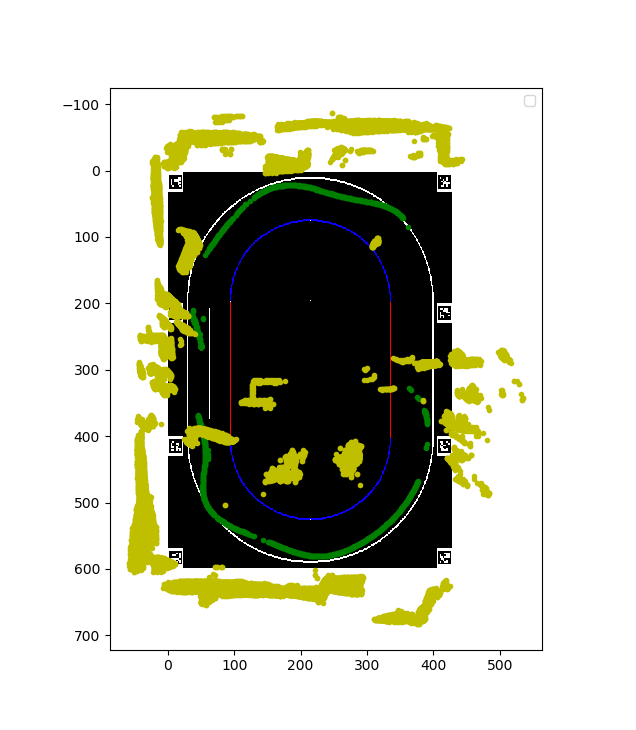
\includegraphics[scale=0.7]{pictures/circle_with_car_and_obstacles.png}
      \caption{Karte mit Lokalisationen des Autos (grün) und erkannte Objekte des lidars (gelb). }
    \end{figure}
    Quellcode: \\
    \url{https://github.com/bigzed/model_car/blob/version-4.0/texinput/src/localization.py} \\
    Video: \\
    \url{https://github.com/bigzed/model_car/blob/version-4.0/texinput/videos/U11_video2.MP4}
	\begin{itemize}
	    \item Wir benutzen 1.5 m als Distanz für den lidar sensor.
	    \item Da die Odometriedaten von der Lokalisierung mit großer Verzögerung ankamen, gibt es die Lücken wie oben gezeigt auf dem Plot.
	    \item Auf der Grafik erkennt man, dass das Auto auf der linken Linie vor dem obstacle auf zwei Linien zum Halt gekommen war. Auf der rechten Linie kann man sehen, dass dort ein obstacle war, diesem ist das Auto ausgewichen. Auf dem oberen Kreis, war ein weiteres obstacle, diesem ist das Auto ausgewichen und ist rechts rum gefahren. 
	\end{itemize}
	\newpage
	\begin{enumerate}
	    \item Für die Transformation benutzen wir tf.transformations mit TransformBroadcaster und sendTransform und TransformListener sowie transformPoint. Dann rechnen wir in die anderen Koordinaten um.
	    \item Wir benutzen die Funktion closest point von Übungsblatt 9 mit einigen Änderungen an der Funktion für die Bereiche im Kreis. Dann berechnen wir einen closepoint relativ zum Punkt. Wir behalten einen Einheitsvektor vom Auto und merken uns die Richtung von diesem Richtungsvektor vom Auto. Ein weiterer Vektor zeigt auf den Kreismittelpunkt. Mithilfe der Vektoren zwischen Auto und closest point und Auto und Kreismittelpunkt und Einheitsvektor erhalten wir wir den Winkel.
	    \item In unserer laneisfree Funktion benutzen u. a. die closest point Funktion mit Eingabe der Punkte von der point cloud und überprüfen somit, ob ein Punkt auf der lane liegt.
	    \item Wir benutzen die laneisfree Funktion von 3. und übergeben dieser die lane auf der wir gerade fahren. Falls kein obstacle gefunden wurde, publish die Geschwindigkeit. Falls ein obstacle gefunden wurde dann setze die andere lane als aktuell. Falls keiner dieser beiden Fälle eintritt, dann ist ein obstacle auf beiden lanes und wir publishen die Geschwindigkeit 0.
	\end{enumerate}
    
	\newpage
	
\end{document}
